\clearpage
\section{Observed-object support, part geometry and complete-policy tests}
\label{sec:observed-object-parts}

\paragraph{Shared object support.}
The previous decomposition motivates an explicit restriction of the completion model's domain. Variant O constructs one box/shelf pair per acquired positive instance track and removes unassociated fragments from hypothetical furniture completion. All measured map points, generic measured-quality rewards, unknown-coverage scores and candidates remain. This changes the research model, rather than being an equivalent engineering implementation. G and S receive the same ideal visible instance support; G has a neutral structural-class prior and is not a completely semantics-free frontend. O retains the inherited $0.12<z<1.8$~m input crop and shape initializer. O$_{\rm full}$ restores all already acquired points assigned to those tracks. OF uses this same full support to estimate outer planes from point positions and depth-validated viewing directions. Unobserved endpoints retain the original extent priors. Figure~\ref{fig:observed-template-envelopes} exposes both the missing input support and remaining placement errors.

\paragraph{Two further part-model revisions.}
A requires observed outer-boundary and outward-view support before a vertical plane determines orientation; otherwise the zero-yaw prior remains. B preserves the three inherited slabs' absolute prior heights and constrains observed faces using acquired two-dimensional horizontal patches. Unpaired faces retain the 0.08~m thickness prior; compatible opposite faces constrain thickness. Overlapping intervals are merged, while unconstrained slabs remain, including those above the estimated box/leg height. The fixed plane tests require 2.5~cm residual tolerance, four points and 15~cm horizontal spans. Hidden lateral extents remain unresolved. A-only, B-only and A+B share OF's full acquired support. Their changed hypothetical area is kept separate from the measured TSDF, with no new reward coefficient, candidate rule or stop condition.

\paragraph{Matched diagnostic outcomes.}
Every variant reuses the same six prefixes and 66 acquired outbound branches from Section~\ref{sec:staged-template-geometry}. No new branch is acquired and no additional independent sample is claimed. Input points, normals and labels match by ordered hashes; reconstructed prefix meshes match byte for byte. The evaluator alone accesses reference object surfaces. O preserves every previously assigned positive track and the preceding pooling variant's pointwise forecasts for those tracks, while removing only unassociated furniture hypotheses. Some acquired points near actual furniture remain unassigned by the frontend; they stay in the measured map and are not relabeled using the reference.

\begin{table}[!htbp]
\centering\small\setlength{\tabcolsep}{4.0pt}
\caption{Observed-object and part-geometry diagnostics on the same six prefixes and 66 reused branches. O uses acquired tracks; O$_{\rm full}$ restores cropped points; OF fits envelopes; A qualifies outside-plane orientation; B fits absolute slab heights. $U$/$V$ are candidate-mean weights supported by actual furniture surfaces/newly realized after acquisition, in m$^2$. These alternative-hypothesis integrals are not unique physical area. $\rho$ correlates predicted reward with actual object net increment within each state. The last three columns report selected-candidate net object/global area and actions. State means receive equal weight; no additional branch executions or independent samples are added.}
\label{tab:observed-object-parts-diagnostic}
\begin{tabular}{llrrrrrr}
\toprule
Stage & Arm & $U$ & $V$ & $\rho$ & $\Delta A_o$ (m$^2$) & $\Delta A_g$ (m$^2$) & Actions \\
\midrule
O & G & 0.216 & 0.124 & 0.848 & 1.050 & 15.792 & 39.5 \\
 & S & 0.164 & 0.086 & 0.848 & 1.057 & 15.968 & 40.2 \\
O$_{\rm full}$ & G & 0.214 & 0.123 & 0.849 & 1.050 & 15.792 & 39.5 \\
 & S & 0.162 & 0.084 & 0.848 & 1.057 & 15.968 & 40.2 \\
OF & G & 0.237 & 0.090 & 0.788 & 1.161 & 13.949 & 38.3 \\
 & S & 0.163 & 0.049 & 0.800 & 1.168 & 14.125 & 39.0 \\
\midrule
OF+A & G & 0.244 & 0.104 & 0.807 & 1.161 & 13.949 & 38.3 \\
 & S & 0.176 & 0.051 & 0.819 & 1.161 & 13.949 & 38.3 \\
OF+B & G & 0.274 & 0.097 & 0.794 & 1.168 & 14.125 & 39.0 \\
 & S & 0.232 & 0.071 & 0.758 & 1.168 & 14.125 & 39.0 \\
OF+A+B & G & 0.292 & 0.109 & 0.811 & 1.168 & 14.125 & 39.0 \\
 & S & 0.262 & 0.073 & 0.791 & 1.168 & 14.125 & 39.0 \\
\bottomrule
\end{tabular}
\end{table}


O's mean within-state rank correlation is approximately 0.848 for both G and S. Restoring cropped points alone does not change any selected candidate. OF lowers S's newly realized true-object prediction weight from 0.0857 to 0.0489~m$^2$ and rank correlation from 0.848 to 0.800. A+B increases realized weight to 0.0729~m$^2$, whereas rank correlation decreases further to 0.791. Supported weight also increases relative to OF, but realized weight and ranking remain below O. A-only and B-only are also retained in Table~\ref{tab:observed-object-parts-diagnostic}. For all three A/B revisions, G and S select the same candidate at every state. The selected A+B branches trade more object recovery for less global recovery than O; their mean shelf recall rises while cabinet recall falls. None is promoted to a complete-policy test. Across all 12 object/state fits, the depth estimate still uses the 0.65~m prior rather than two observed opposing faces. These are development findings on repeatedly inspected states, not held-out shape-generalization evidence.


\paragraph{Observed-data depth identifiability.}
A final frozen diagnostic profiles local object depth while holding all other A+B parts fixed. It compares 21 depths from the measured span to 1.3~m, plus the current prior, using the same acquired valid-depth rays for every candidate and a neutral box/shelf mixture. Surface discrepancy and verified-free contradiction form a heuristic cost $J(d)$; the predeclared plausible band is $J(d)\leq\min J+1$, not a confidence interval. Of 12 object/state pairs, eight lack a unique observed endpoint. All four eligible curves prefer the measured-span lower bound, but the 0.65~m prior remains inside the band: its cost gaps are 0.351--0.676. Thus the measurements contain a depth preference, but this estimator cannot exclude the prior under the fixed rule. No dimension is proposed or updated. The G/S model arrays remain exactly equal to frozen A+B outputs; no candidate scoring, branch acquisition or closed-loop run is repeated. This does not establish that the sensors contain no usable size information.

\begin{figure}[!htbp]
\centering
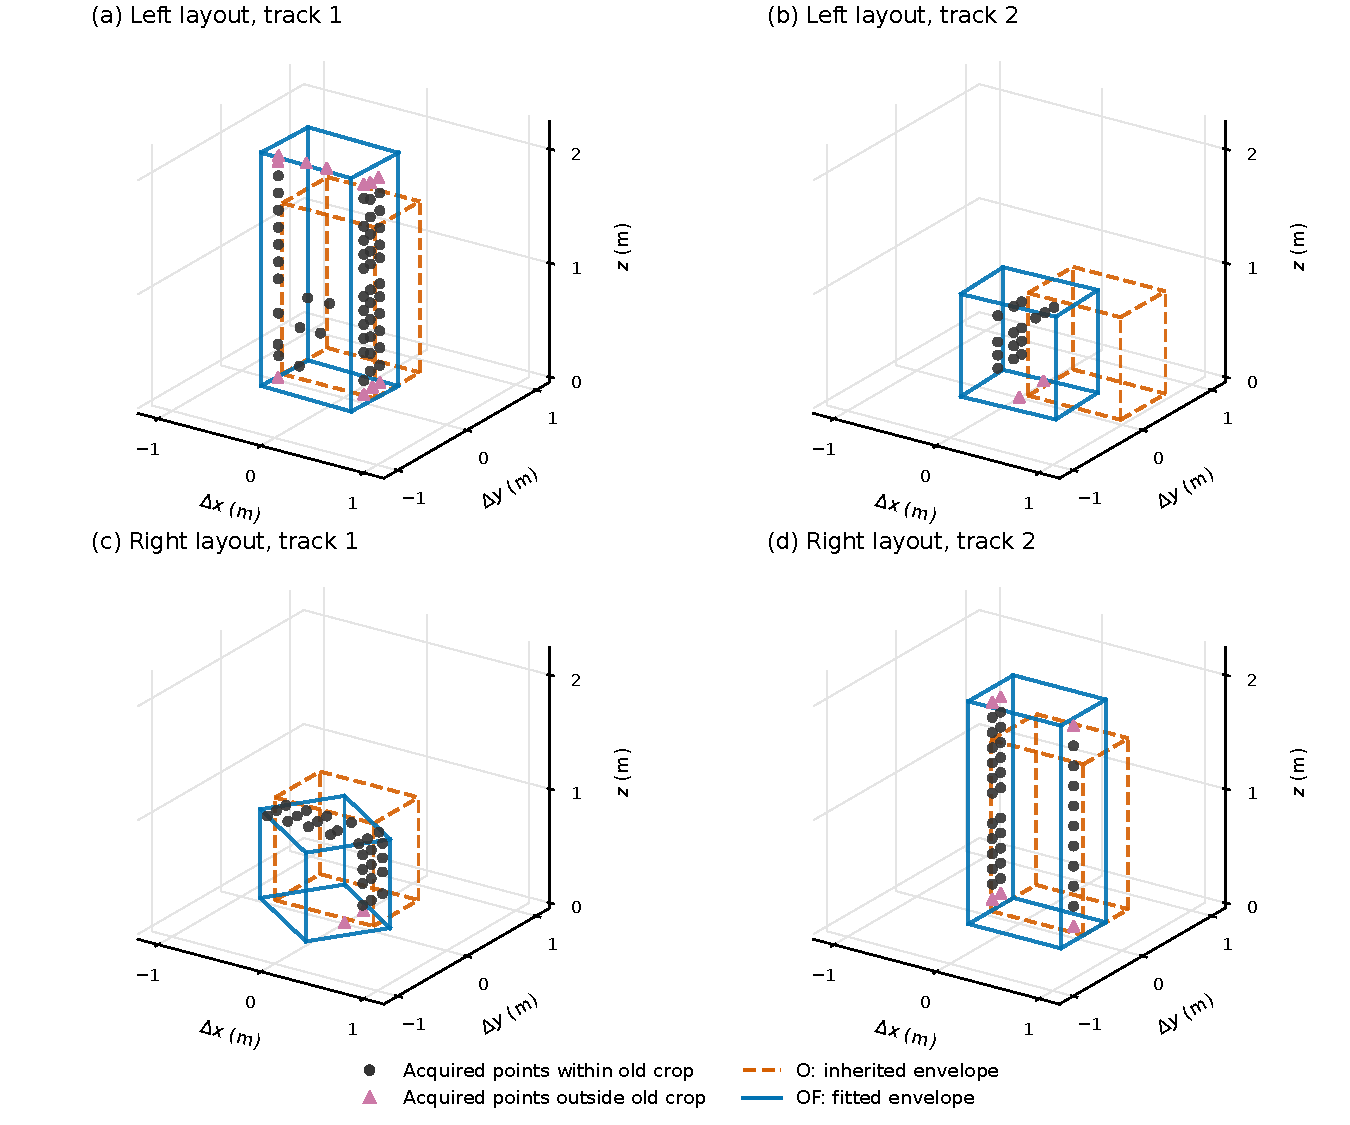
\includegraphics[width=0.87\linewidth]{figures/observed_points_template_envelopes.pdf}
\caption{Acquired points and predicted envelopes at the preselected 24-action prefixes. Black points fall inside the old input height crop; purple triangles are already acquired points outside it. Dashed orange and solid blue outlines show O and OF, respectively. Both tracked objects in each layout are shown, including the rotated fit in (c). Axes share a metric scale; horizontal origins are observed-point centroids and height is relative to the simulated ground. The outlines are shared template envelopes, not complete measured reconstructions or evidence of unseen-surface accuracy.}
\label{fig:observed-template-envelopes}
\end{figure}

\subsection{O-only closed-loop comparison and isolated ablations}
O is tested in a separately frozen eight-run matrix: G, S, S$^{-\ell}$ and S$^{-m}$ in both existing layouts. S$^{-\ell}$ removes only the original measured surface-distance likelihood from the structural posterior; it does not remove the category prior or change template placement. S$^{-m}$ removes only measured-surface reward consumption, retaining strict valid-free rejection. All other inputs, scoring terms, candidates, 256-action budgets and return rules are shared. All eight runs complete correct-free coverage, return and record zero simulated collisions (Table~\ref{tab:observed-object-policy}). This supports controlled exploration feasibility, with the outcomes below limiting the claim of semantic benefit.

\begin{table}[!htbp]
\centering\small\setlength{\tabcolsep}{4.0pt}
\caption{Complete O-policy matrix on the two existing furniture permutations. All eight runs reach 100\% correct-free coverage, return, use 256 paid actions and record zero simulated collisions. Both G and S receive the same ideal acquired instance support; only their structural-class prior differs. S$^{-\ell}$ disables only the inherited measured-distance likelihood, whereas S$^{-m}$ disables only measured-surface reward consumption and retains verified-free rejection. $a_{100}$ is the first full-coverage action; $d$ is full-budget path length. $R_o$/$R_c$ denote open-shelf/closed-cabinet recall at 5~cm. These are eight deterministic runs of four policies on one floorplan family, not eight independent environments or repeats.}
\label{tab:observed-object-policy}
\begin{tabular}{llrrrrrr}
\toprule
Layout & Mode & $a_{100}$ & $d$ (m) & F1$_5$ (\%) & F1$_{10}$ (\%) & $R_o$ (\%) & $R_c$ (\%) \\
\midrule
Left & G & 88 & 42.0 & 92.76 & 94.00 & 82.17 & 88.71 \\
 & S & 97 & 43.2 & 92.38 & 93.80 & 83.46 & 85.87 \\
 & S$^{-\ell}$ & 97 & 43.2 & 92.38 & 93.80 & 83.46 & 85.87 \\
 & S$^{-m}$ & 97 & 43.6 & 92.46 & 93.79 & 83.28 & 86.13 \\
\midrule
Right & G & 100 & 43.2 & 92.60 & 93.88 & 81.09 & 79.21 \\
 & S & 100 & 43.2 & 92.60 & 93.88 & 81.09 & 79.21 \\
 & S$^{-\ell}$ & 100 & 43.2 & 92.60 & 93.88 & 81.09 & 79.21 \\
 & S$^{-m}$ & 100 & 43.2 & 92.45 & 93.88 & 80.23 & 79.21 \\
\bottomrule
\end{tabular}
\end{table}


In the left layout, S reaches full coverage nine actions later than G (97 versus 88), travels 1.2~m farther, and loses 0.377 percentage points of terminal 5~cm F1. Shelf recall increases by 1.294 points, while cabinet recall decreases by 2.834 points. The right-layout G/S trajectories and native meshes remain identical. The first left-layout choice difference occurs at planning action 54, and execution first differs at action 71. A per-component audit traces the score change mainly to the cabinet completion: the compared cabinet-forecast points have zero support within 5~cm of the actual cabinet surface. A category prior can therefore amplify a misplaced geometric hypothesis; a changed decision is insufficient evidence of improved information gathering.

S and S$^{-\ell}$ have identical trajectories and native meshes in both layouts. Thus the inherited likelihood has no observed policy-level effect in this matrix. Consumption also has mixed effects: removing it raises left-layout F1 by 0.076 points with 0.4~m additional path and slightly lower shelf recall; on the right it lowers F1 by 0.147 points and shelf recall by 0.858 points. These outcomes differ from the earlier full-basis consumption contrast because the model domain and resulting policy have changed. Historical cap-free B2, C and J outcomes remain reused controls, not new runs or independent scenes. The eight new deterministic runs add neither natural-detector validation nor physical SLAM evidence.
